%------------------------------------------------------------------------
% Chapter:  Simple crystal modifications
%------------------------------------------------------------------------

\chapter{Simple crystal modifications \label{mod-simple}}

Chapter \ref{struc} discussed techniques to create a 
perfect model crystal from the content of the asymmetric unit.
This chapter will give an overview of simple modifications of single
atoms within a model crystal.  Section \ref{mod} will describe
\Discus tools to modify a complete crystal.

%------------------------------------------------------------------------

\section{Modifications using variables \label{mod-var}}

Each atom $<$i$>$ within the model crystal stored by the program
\Discus is associated with a set of variables x[$<$i$>$],
y[$<$i$>$] and z[$<$i$>$] that describe its position and the variable
m[$<$i$>$] that contains the atom type (see also section \ref{get}). In
principle every desired defect structure might be realized using
these variables and the FORTRAN style loops and conditional
statements (see chapter FORTRAN style interpreter in the 
package manual). One should be aware that this
procedure may be very slow for complex problems and large model
crystals.  Since the variables are addressed using the atom index
$<$i$>$, a knowledge about the internal storage as described in
section \ref{struc-int} is very important.  The command {\tt trans}
in the 'chem' segment of \Discus allows one to convert between
atom index and the corresponding unit cell and site. To illustrate
the use of variables, the following type of defect should be
constructed using \discus. The starting structure is a 10x10x1
unit cell square symmetric crystal with Zr on (0,0,0) and a lattice
constant of a=5\AA. The defects consist of randomly introduced
vacancies on Zr sites and nearest neighbors surrounding the vacancy
should be relaxed towards the vacant site. The perfect starting
structure and the resulting disordered structure are shown in figure
\ref{mod1-fig1}.
%
\begin{figure}[htb]
   \centering
   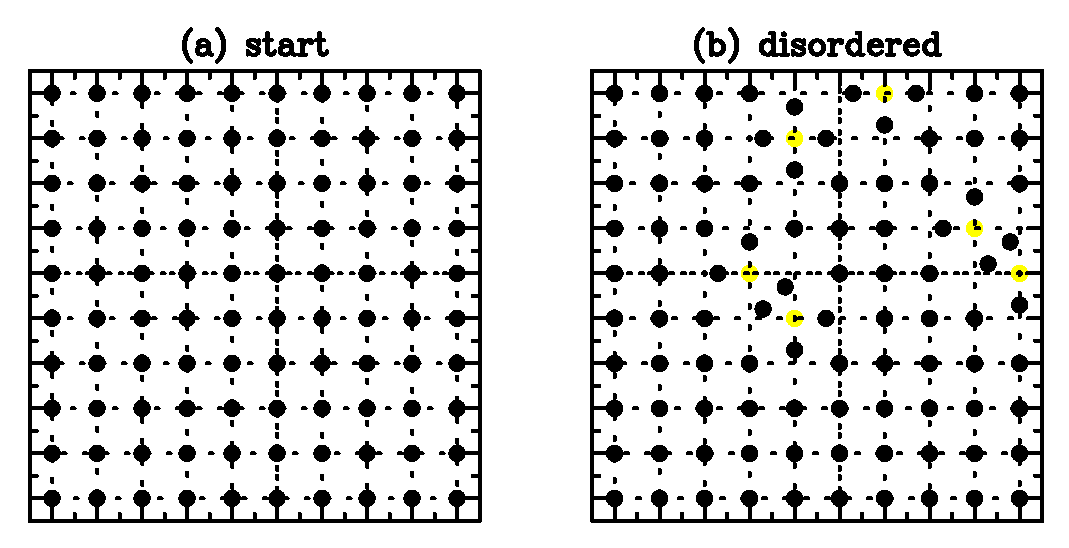
\includegraphics[scale=0.9, angle=0]{mod1.1.eps}
   \caption{Structures created by crystal modification example}
   \label{mod1-fig1}
\end{figure}
%
Here is the macro used to create the described defects.  Again the
line numbers are only shown for convenience and not part of the
macro itself. To achieve a high degree of flexibility values like
crystal size or the number of defects to be created are stored in
variables at the beginning of the macro.  The desired crystal size
is stores in variables i[1], i[2] and i[3] (lines 1-3).  The
variable i[4] (line 5) gives the number of defects to be created
and r[1] (line 6) specifies the relaxation (here 30 \%) of the
surrounding neighbors towards the vacant site.
%
\begin{MacVerbatim}
     1  i[1] = 10
     2  i[2] = 10
     3  i[3] = 1
     4  #
     5  i[4] = 6
     6  r[1] = 0.30
     7  #
\end{MacVerbatim}
%
Next we read the unit cell from file {\it cell.cll} and expand it to
the desired size (lines 8-9).  The macro {\it plot.mac} (line 11)
saves the starting structure suitable for plotting with {\it KUPLOT}
as seen in figure \ref{mod1-fig1}a).
%
\begin{MacVerbatim}
     8  read
     9  cell cell.cll,i[1],i[2],i[3]
    10  #
    11  @plot before.plot
    12  #
\end{MacVerbatim}
%
The next part (lines 13-15) is needed to switch off periodic crystal
boundaries for the command {\tt find} (line 24), otherwise our
simple way of relaxing the neighbors would not work.
%
\begin{MacVerbatim}
    13  chem
    14  set mode,quick,noperiodic
    15  exit
\end{MacVerbatim}
%
Now the creation of the disordered structure starts with a loop over
the number of defects to be created (line 19).  Next a crystal site
is chosen at random (line 20).  Note that the function {\tt ran(0)}
produces a random number between 0 and 1 which is multiplied with
the number of atoms within the crystal (n[3] contains the number of
atoms per unit cell, see table \ref{v1-tab} in section \ref{get}).  
If an occupied site
was picked (line 22) the atom is removed (line 23).  The command
{\tt find} (line 24) returns all atoms of the type Zr around the
position of the selected site within a radius of 5.5\AA.  The atom
indices of these nearest neighbors are stored in the variables {\tt
env[$<$i$>$]} and {\tt env[0]} contains the number of found
neighbors. Finally the positions of all neighboring atoms returned
by {\tt find} are moved towards the vacant site (lines 27-29).
%
\begin{MacVerbatim}
    16  #
    17  # Loop number of wanted defects
    18  #
    19  do i[5]=1,i[4]
    20    i[6]=int(ran(0)*i[1]*i[2]*i[3]*n[3])+1
    21  #
    22    if(m[i[6]].eq.1) then
    23      m[i[6]]=0
    24      find env,zr,x[i[6]],y[i[6]],z[i[6]],5.5
    25  #
    26      do i[7]=1,env[0]
    27        x[env[i[7]]]=x[env[i[7]]]-r[1]*(x[env[i[7]]]-x[i[6]])
    28        y[env[i[7]]]=y[env[i[7]]]-r[1]*(y[env[i[7]]]-y[i[6]])
    29        z[env[i[7]]]=z[env[i[7]]]-r[1]*(z[env[i[7]]]-z[i[6]])
    30      enddo
    31  #
    32    endif
    33  #
    34  enddo
    35  #
    36  @plot after.plot
\end{MacVerbatim}
%
The resulting structure can be seen in figure \ref{mod1-fig1}b.
The introduced vacancies are shown as yellow circles (or light
grey). Since this simple macro does not check whether neighboring
atoms are already displaced, the clustered defects in the upper
right quadrant of figure \ref{mod1-fig1}b have a different local
environment compared to the isolated defects.

%------------------------------------------------------------------------

\section{Build in functions \label{mod-buildin}}

This section will give an overview of those \Discus functions
modifying single atoms or molecules.  Some of these functions can be
realized using variables as well, others cannot like the command
{\tt insert} to insert a new atom in the model crystal.  Table
\ref{mod-tab-1} summarizes the available commands.
%
\begin{table}[!tbh]
\centering
\begin{tabularx}{\textwidth}{|p{30mm}|X|}
  \hline
  {\bf Command} & {\bf Description} \\
  \hline\hline
  append  & Appends an atom at a given position within the crystal if
            no other atoms are present in a given distance.\\
  copy    & Copies an atom to a different position given absolute or
            relative to the other position.\\
  insert  & Inserts a new atom at the given position without condition.\\
  kick    & Inserts a new atom at a given position and removes all
            other atoms within a given distance from the new atom.\\
  remove  & Removes an atom or molecule from the crystal.\\
  switch  & Swaps two given atoms or molecules within the crystal.\\
  purge   & Removes vacancies (VOID) from the crystal ({\bf use with
            care})\\
  replace & Replaces one or more atoms or molecules with the given
            type.\\
  \hline
\end{tabularx}
\caption{\label{mod-tab-1}\Discus commands for single atoms or
         molecules}
\end{table}
%
Basically there are three commands to insert a new atom in the
structure. The command {\tt insert} just creates a new atom at a
specified position without taking notice of its environment. Thus
the new atom might be on top of an existing one. In order to avoid
this problem, \Discus provides two other commands {\tt append}
which will not insert the atom if there are other atoms within a
given distance and {\tt kick} which will remove those atoms close by
before inserting the new one. The command {\tt copy} allows the user
to copy an existing atom to a new position that can be given in
absolute coordinated or relative to the position of the atom to be
copied. Note, that these commands are limited to atoms. New molecule
types can be created and molecules copied using the generalized
symmetry segment of \Discus described in chapter
\ref{cryst-sym}. \par

The commands {\tt remove} and {\tt switch} work for atoms as well as
molecules. Not surprisingly, {\tt remove} removes an atom or
molecule and {\tt switch} swaps two atoms or molecules with respect
to their location within the crystal. \par

The commands mentioned in this section so far operate only on a
single atom or molecule. The command {\tt replace} can replace a
single atom or molecule by a given type or replace more until a
given concentration is reached. Although this can be easily realized
using the FORTRAN interpreter and variables associated with the
crystal, the internal function is much faster, especially for large
crystal sizes. The command {\tt purge} will remove all vacancies
(VOID) within the crystal. Note that if you remove an atom or a
molecule by the {\tt remove} command, \Discus will not actually
remove atoms but rather replace their atom type with VOID. Thus when
saving the structure a large number of VOID's might appear in the
number. The use of {\tt purge} actually removes those VOID atoms.
However, the use of the {\tt purge} command is {\bf not recommended}
since many \Discus function require the crystal to be build in
a given order, i.e. having the same number of atom sites within
every unit cell either occupied by an atom or a VOID.

%------------------------------------------------------------------------

\section{Inserting extended objects \label{mod-insert}}

In order to insert extended objects for small angle scattering or
domains \ref{mod-domain} \Discus offers an insert menu. In contrast
to the insert command for individual atoms, the menu is evoked by
the {\tt insert} command followed by the keyword {\tt domain} or
{\tt object}. A corresponding version for molecules is under
construction. 

\subsection{Inserting domains \label{mod-insdom}}

Within the \Discus formalism, a domain (see section 
\ref{mod-domain} for a full explanation ) is 
essentially a molecule which will be interpreted differently. 
The domain allows you to place an extended defect into a host 
structure. The {\tt insert domain} menu allows you to specify
the character and location of the domain to be inserted.


%------------------------------------------------------------------------

\section{Building   a molecule \label{mod-molec}}

To build a molecule or to extend an existing molecule, \Discus
offers the {\tt molecularize} command. 
\begin{MacVerbatim}
 1 molecularize conn, <central> [, <exclude> ...]
 2 molecularize range, <from>, <to>, <molecule_type> , <molecule_Biso>
\end{MacVerbatim}

The first command version builds molecules for the central atom
number  <central>. Prior to this command a connectivity list must have been
created with the help of the connectivity menu. This connectivity list is
searched to find all neighbors to the central atom type and the resulting
further neighbors in turn. The list of excluded atom number can be used 
to prevent these excluded atom to become part of the molecule. 
This allows you to build a partial molecule, which could be helpful
if a section of a molecule needs to be turned with respect to the rest.

The second command form combines all atoms from number <from> to number <to>
into a singel molecule. \discus does not check if these atoms are close to 
each other.

%------------------------------------------------------------------------

\section{Dissolving a molecule \label{mod-demole}}

Under rare cirumstances it might be advantageous to {\it dissolve} a molecule.
The idea is to remove all molecule info, while retaining the atoms that are in
the molecule at their original place with all other but molecule related 
properties to remain the same. The instructions for this task are bundled in
the "demolecularize" menu.

\begin{MacVerbatim}
 1 demolecularize
 2   reset
 3   select moletype:all,atomtype:none
 4   include molerange:all, atomrange:none
 5   property {"ignore"|"present"|"absent"} , <property> [, <property> ...]
 6   show
 7   run
 8 exit
\end{MacVerbatim}

The "select" and "include" commands on line 3 and 4 are the two main instructions
for this menu. "select" allows you to chose, which molecule types are to be 
dissolved. Possible values for the parameter are:

\begin{tabularx}{\textwidth}{|p{30mm}|X|}
  \hline
  {\bf Parameter} & {\bf Description} \\
  \hline\hline
  none    & No  molecule type  will be dissolved. Default\\
  all     & All molecule types will be dissolved.\\
  <n1>    & Only molecule of type <n1> will be dissolved.\\
  (<n1>,<n2>{,...})    & All  molecule of the specified types 
                         will be dissolved. The list needs to be enclosed in
                         round parentheses.\\
  \hline
\end{tabularx}

The "include" command defines which numerical range of molecules shall be 
dissolved. 

\begin{tabularx}{\textwidth}{|p{30mm}|X|}
  \hline
  {\bf Parameter} & {\bf Description} \\
  \hline\hline
  none    & No range of molecules will be dissolved. Default\\
  all     & All molecule numbers will be dissolved.\\
  <n1>    & Only the molecule number  <n1> will be dissolved.\\
  (<n1>,<n2>)    & All  molecules in the range from <n1> to <n2>
                         will be dissolved. If <n1> is equal to -1 or 
                         "last", all molecules from number <n1> to the 
                         last molecule will be dissolved. The list needs to be 
                         enclosed in round parentheses.\\
  \hline
\end{tabularx}

The two commands work together as a logical AND. Only molecules that are in the
list of molecule types and that fall in the range of molecule numbers will be
dissolved.

To specify even more details, the selection and inclusion can be more fine tuned
with the "atomtype" and "atomrange" parameters.

The atomtype accepts the following parameters:

\begin{tabularx}{\textwidth}{|p{30mm}|X|}
  \hline
  {\bf Parameter} & {\bf Description} \\
  \hline\hline
  none    & The atoms in the molecule do not have to be of a specific type for
            the molecule to be dissolved. A molecule may consist of any atom 
            type(s). Default\\
  all     & A molecule must contain all atom types to be dissolved. If a 
            molecule is missing any atom type it will not be dissolved. \\
  <n1>    & A molecule must contain at least one atom of type <n1> to be 
            dissolved. Other atom types may be present as well and do not affect
            the decision. \\
  (<n1>,<n2>{,...})    & A molecule must contain at least one atom of each of 
                         the specified types to be be dissolved. The list needs
                         to be enclosed in round parentheses.\\
  \hline
\end{tabularx}

The "atomrange" command accepts the following parameters:

\begin{tabularx}{\textwidth}{|p{30mm}|X|}
  \hline
  {\bf Parameter} & {\bf Description} \\
  \hline\hline
  none    & No specific range of atoms needs to be present in a molecule for 
            it to be dissolved. Default\\
  all     & Any molecule must contain all atoms from number 1 to the last to be 
            dissolved. \\
  <n1>    & The molecule must contain exactly the atom number <n1> in order to 
            be dissolved.\\
  (<n1>,<n2>)    & All atoms in the molecule must fall into the range from <n1> 
                   to <n2> for the molecule to be dissolved. It is not necessary
                   that the entire range is covered. The condition states that 
                   if any atom in the molecule is outside the range from <n1> 
                   to <n2> the molecule will not be dissolved. If <n1> is equal 
                   to -1 or "last", all molecules from number <n1> to the 
                   last molecule will be dissolved. The list needs to be 
                   enclosed in round parentheses.\\
  \hline
\end{tabularx}

The local properties set with the "property" command define, which properties 
all atoms in a given molecule must have for this molecule to be demolecularized.
The properties default to "ignore", which means that an atom may have any
property, without affecting the choice for the given molecule.

Both, the "atomtype" and "atomrange" and the property selection impose 
conditions that must be met, they
are interpreted as a logical AND with the "moletype" and "molerange" parameters.

\section{Creating a periodic structure \label{mod-per}}

Under several circumstances, the current structure might not be periodic or at least 
might not correspond to the sequence of atoms and unit cells as generated upon the 
expansion of an asymmetric unit, see chapter \ref{struc}. A simple
example might be the structure after you purged vacancies. Other more involved
examples might result from the introduction of domains, see \ref{mod-domain}, or
if the crystal was build using stacking faults, see \ref{mod-stack}. Finally, the 
sequence of atoms generated for other programs like RMCprofile, molecular dynamics 
programs or DFT like programs will likely be different from the sequence use 
by \discus.

For fast calculations within \Discus it is often desireable to have the atoms
arranged in the strict sequence as generated in chapter \ref{struc}. This 
sequence allow \Discus to find neighboring atoms much faster as the search is 
restricted to a few unit cells. These searches are perfomed at many parts of 
the program. It is thus desireable to be able to sort the atoms of a given 
structure in this standard sequence. 

The {\tt perioditize} menu has been designed to perform this task. Under 
opportune circumstances it will do the job completely automatically, but it 
will most likely to 
be helped by providing information such as the number of unit cells, the 
number of atoms per unit cell and the sites within the unit cell.

A simple macro to perform the task might be:

\begin{MacVerbatim}
1  perioditize
2    set ncell, 3,4,5
3    set natoms, 8
4    run
5  exit
\end{MacVerbatim}

The {\tt ncell} command defines that the crystal consists of the given 
number of unit cells along the three axes. The {\tt natoms} command defines the
number of atoms per unit cell. As no {\tt set pos} command is given, 
the program will attempt to automatically establish the actual positions 
within the average unit cell. 

The task is much simpler if the user specifies the actual sites within the 
average unit cell. this can be done within the {\tt perioditize} menu
with 
\begin{MacVerbatim}
1  set site, atoms:[names], pos:[x,y,z], number:value
\end{MacVerbatim}
Both, the {\tt atoms:} and the {\tt pos:} parameters are required. The
{\tt atoms:} parameter defines which atom types may occupy the given site. 
Atom names can be spcifies as list of current atom names or alternatively 
as the string {\tt all} to imply all atom types. The parameters to the 
{\tt pos} parameter must specify fractional coordinates in the range [0,1].
The {\tt number} parameter is optional and mainly serves to correct 
previous settings.

In case of a structure with many symmetrically equivalent sites, it will
be more compfortable to use the equivalent command:
\begin{MacVerbatim}
1  set wyck, atoms:[names], pos:[x,y,z]
\end{MacVerbatim}
In contrast to {\tt set site} this version creates all symmetrically 
equivalent Wyckoff sites for the position [x,y,z]. It uses the current 
space group. As several sites will be generated, {\tt set wyck} does not
use the {\tt number:} parameter, and the new sites will be placed into
the next free spaces. 

There are many cases under which a structure cannot be rearranged in a
periodic fashion since the underlying actual structure simply is not
periodic or differs too widely for the current algorithm to cope. 
Examples include:

\begin{tabularx}{\textwidth}{|p{30mm}|X|}
  \hline
  {\bf Example} & {\bf Description} \\
  \hline\hline
  amorphous    & A truly amorphous structure such as a glass or liquid 
                 cannot be expressed as a periodif structure. \\
  composite    & A structure that consists of blocks with different 
                 internal lattice parameters. This could be an inclusion
                 compound or a layered structure.\\
  core/shell   & Nanaoparticles whose core differs in its structure
                 from the shell.\\
  stacks       & The result of stacking faults will in most cases yield
                 an inherently non-periodic structure. This holds in 
                 particular if the translation vectors are not simple
                 rational numbers. \\
  finite       & For a finite object created with the surface menu large
                 fractions might be missing. These can only be reconstructed
                 if the full site, unit cell number and atoms per unit 
                 cell is given.\\
  \hline
\end{tabularx}
%------------------------------------------------------------------------
